\documentclass[a4paper, 12pt]{article}
\usepackage[utf8]{inputenc}
\usepackage[english,russian]{babel}
\usepackage[warn]{mathtext}
\usepackage{graphicx}
\usepackage{float}
\usepackage{multirow}
\restylefloat{table}
\usepackage{amsmath}
\usepackage{floatflt}
\usepackage[T2A]{fontenc}
\usepackage[left=20mm, top=20mm, right=20mm, bottom=20mm, footskip=10mm]{geometry}

\tolerance 1414
\hbadness 1414
\emergencystretch 1.5em
\hfuzz 0.3pt        % размер максимального переполнения без warning'a
\widowpenalty=10000 % запрещает одиночную строку абзаца в начале страницы
\vfuzz \hfuzz
\raggedbottom       % если на странице мало содержимого, добавить пустое место в конце, а не в середине страницы



\begin{document}

\begin{titlepage}
	\centering
	\vspace{5cm}
	{\scshape\LARGE московский физико-технический институт (национальный исследовательский университет) \par}
	\vspace{6cm}
	{\scshape\Large Лабораторная работа 5.1 \par}
	{\huge\bfseries Экспериментальная проверка уравнения Эйнштейна для фотоэффекта и определение постоянной Планка \par}
	\vspace{1cm}
	\vfill
\begin{flushright}
	{\large Б03-104}\par
	\vspace{0.3cm}
	{\LARGE Куланов Александр}
\end{flushright}
	

	\vfill


	Долгопрудный, 2023 г.
\end{titlepage}

\begin{itemize}
	\item \textbf{Цель работы:} исследовать зависимость фототока от величины задерживающего потенциала и частоты падающего излучения и вычислить величину постоянной Планка
\end{itemize}

\section{Теоретические сведения}

Фотоэффект --- явление испускания электронов фотокатодом, облучаемым светом. На фотокатод падают частицы, 
называемые фотонами, которые обладают энергией $\hbar \omega$ и импульсом $\hbar\omega/c$. 
При столкновении фотона с электроном фотокатода энергия фотона полностью передается электрону, и фотон прекращает свое существование. Энергетический баланс этого взаимодействия для вылетающих электронов описывается уравнением

\begin{equation}
	\hbar \omega = E_{max} + W
	\label{eq:energy}
\end{equation}

Здесь $ E_{max} $ ---  максимальная кинетическая энергия электрона после выхода из фотокатода, $ W $ --- работа выхода электрона из катода.

\begin{figure}[H]
    \centering
    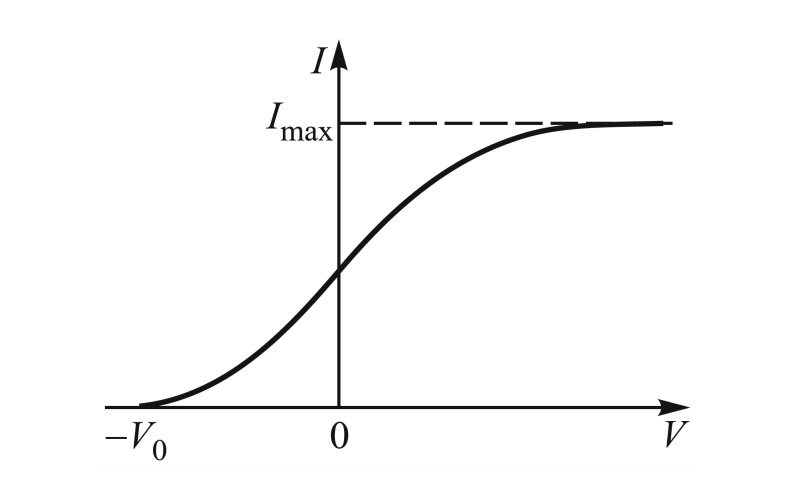
\includegraphics[width=0.5\textwidth]{VI.jpg}
    \caption{Зависимость силы тока от напряжения при фотоэффекте}
    \label{fig:IV}
\end{figure}

Для измерения энергии вылетевших фотоэлектронов обычно располагают второй электрод
(анод), на который подается задерживающий или ускоряющий потенциал. При достаточно больших
ускоряющих напряжениях фототок достигает насыщения (рис. \ref{fig:IV}), то есть все элетроны долетают до анода.

При некотором значении $ V = -V_0 $ (потенциал запирания) никакие электроны не долетают до анода.
Максимальная кинетическая энергия $ E_{max} $ электронов связана с запирающим потенциалом $ V_0 $: $ E_{max} = eV_0 $. Тогда уравнение (\ref{eq:energy}) примет вид, называемый уравнением Эйнштейна:
	
\begin{equation}
	eV_0 = \hbar\omega - W
	\label{eq:Einstein}
\end{equation}

Для определения запирающего напряжения, нужно экстраполировать зависимость тока от нарпяжения к нулю. В нашем случае с аксиальной симметрией корень из тока линейно зависит от запирающего напряжения.
Чтобы это сделать, определяются потенциалы запирания при разных частотах (длинах света) и строится зависимость $V_0(\omega)$. Как следует из (\ref{eq:Einstein}),

\begin{equation}
	\dfrac{dV_0}{d\omega} = \dfrac{\hbar}{e}
	\label{eq:dV/dw}
\end{equation}

То есть по наклону прямой можно определить постоянную Планка.


\section{Экспериментальная установка}
Схема установки представлена на рисунке (\ref{fig:set})

\begin{figure}[H]
    \centering
    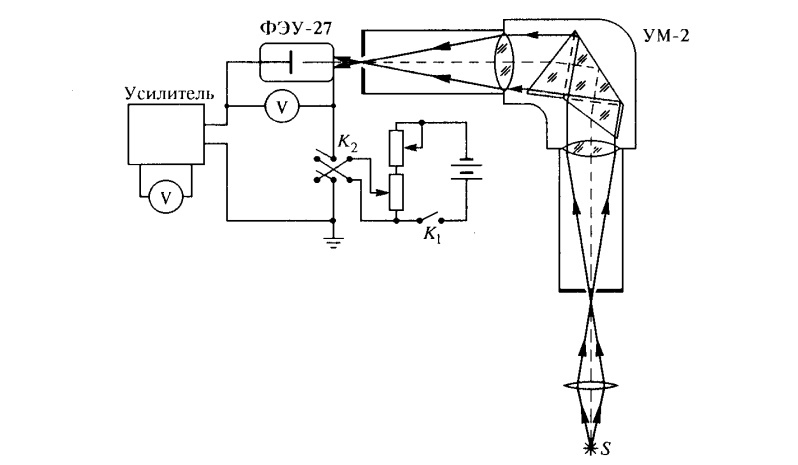
\includegraphics[width=1\textwidth]{set.jpg}
    \caption{Принципиальная схема установки}
    \label{fig:set}
\end{figure}

Свет от источника $S$ (обычная электрическая лампа накаливания) фокусируется на входную щель призменного монохроматора УМ-2, выделяющего узкий спектральный интервал, и попадает на фотокатод фотоэлектронного умножителя ФЭУ. В качестве фотокатода в данном
ФЭУ используется полупрозрачное висмуто-серебряно-цезиевое покрытие. Тормозящий потенциал подается на сетку (плоский металлический электрод), которая используется в качестве анода. Остальные электроды накоротко соединены с сеткой.

Фототок, протекающий в нашем фотоэлементе, мал, особенно при потенциалах $V$, близких к $V_0$, и не может быть измерен непосредственно. Для его измерения используется усилитель постоянного тока. Для уменьшения погрешностей измерений, обусловленных наводками, усилитель фототока смонтирован в одном корпусе с ФЭУ. 
Абсолютные значения фототока нам не нужны, поэтому он измеряется в относительных единицах по вольтметру, подключенного к выходу усилителя. Эти показания пропорциональны величине измеряемого тока. Тормозящий потенциал регулируется при помощи двух потенциометров «Грубо» и «Плавно», установленных на корпусе блока питания установки. Измерение тормозящего потенциала осуществляется в помощью цифрового вольтметра.


Точное измерение тормозящего потенциала произвести очень трудно, и связано это со следующим обстоятельством. Если составить электрическую цепь из различных проводни-
ков, то возникает контактная разность потенциалов, величина которой определяется разностью работ выходов между крайними проводниками. Контактная разность потенциалов может достигать нескольких вольт, это значительно усложняет в такой разнородной цепи измерение разности потенциалов, возникающей за счет других причин. Это же относится и к измерению прилсженной к цепи внешней разности потенциалов.

Контактная разность потенциалов мешает точному определению величины $V_0$, но не оказывает влияния на определение постоянной Планка, которая выражается через производную $d V_0 / d \omega$.
\section{Выполнение работы}
Таблица с данными для калибровки:

\begin{table}[H]
	\centering
	\begin{tabular}{|c|c|}
	\hline
	\textbf{$\lambda$,   A} & \textbf{$\varphi$, deg} \\ \hline
	7032                 & 2950              \\ \hline
	6929                 & 2922              \\ \hline
	6717                 & 2856              \\ \hline
	6678                 & 2845              \\ \hline
	6599                 & 2812              \\ \hline
	6533                 & 2791              \\ \hline
	6507                 & 2779              \\ \hline
	6402                 & 2744              \\ \hline
	6383                 & 2732              \\ \hline
	6334                 & 2716              \\ \hline
	6305                 & 2703              \\ \hline
	6267                 & 2689              \\ \hline
	6217                 & 2666              \\ \hline
	6164                 & 2642              \\ \hline
	6143                 & 2634              \\ \hline
	6096                 & 2616              \\ \hline
	6074                 & 2604              \\ \hline
	6030                 & 2587              \\ \hline
	5976                 & 2563              \\ \hline
	5945                 & 2550              \\ \hline
	5882                 & 2517              \\ \hline
	5852                 & 2500              \\ \hline
	5401                 & 2248              \\ \hline
	5341                 & 2208              \\ \hline
	5331                 & 2193              \\ \hline
	\end{tabular}
\end{table}

График калибровки:

\begin{figure}[H]
    \centering
    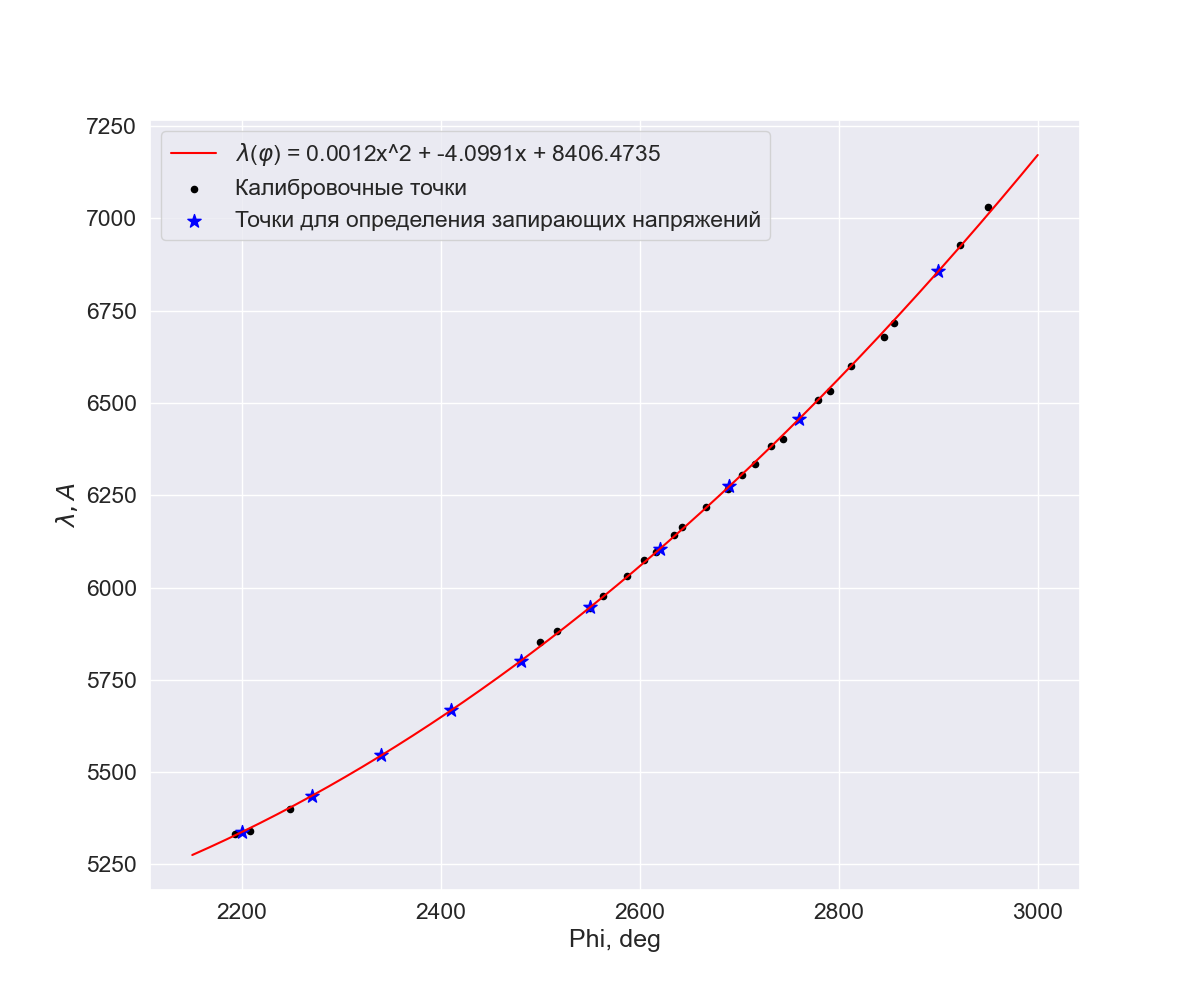
\includegraphics[width=1\textwidth]{plot1.png}
    \caption{График калибровки}
    \label{fig:calib}
\end{figure}

Данные с измерений запирающего напряжения:

\begin{table}[H]
	\centering
	\begin{tabular}{|cc|cc|cc|cc|cc|}
	\hline
	\multicolumn{2}{|c|}{\textbf{2200}}              & \multicolumn{2}{c|}{\textbf{2270}}              & \multicolumn{2}{c|}{\textbf{2340}}              & \multicolumn{2}{c|}{\textbf{2410}}              & \multicolumn{2}{c|}{\textbf{2480}}              \\ \hline
	\multicolumn{1}{|c|}{\textbf{U, V}} & \textbf{I} & \multicolumn{1}{c|}{\textbf{U, V}} & \textbf{I} & \multicolumn{1}{c|}{\textbf{U, V}} & \textbf{I} & \multicolumn{1}{c|}{\textbf{U, V}} & \textbf{I} & \multicolumn{1}{c|}{\textbf{U, V}} & \textbf{I} \\ \hline
	\multicolumn{1}{|c|}{-0,77}         & 0          & \multicolumn{1}{c|}{-0,74}         & 0          & \multicolumn{1}{c|}{-0,72}         & 0          & \multicolumn{1}{c|}{-0,67}         & 0          & \multicolumn{1}{c|}{-0,64}         & 0          \\ \hline
	\multicolumn{1}{|c|}{-0,72}         & 0,03       & \multicolumn{1}{c|}{-0,7}          & 0,02       & \multicolumn{1}{c|}{-0,65}         & 0,04       & \multicolumn{1}{c|}{-0,62}         & 0,04       & \multicolumn{1}{c|}{-0,59}         & 0,03       \\ \hline
	\multicolumn{1}{|c|}{-0,69}         & 0,05       & \multicolumn{1}{c|}{-0,66}         & 0,06       & \multicolumn{1}{c|}{-0,61}         & 0,09       & \multicolumn{1}{c|}{-0,59}         & 0,08       & \multicolumn{1}{c|}{-0,55}         & 0,08       \\ \hline
	\multicolumn{1}{|c|}{-0,63}         & 0,11       & \multicolumn{1}{c|}{-0,6}          & 0,13       & \multicolumn{1}{c|}{-0,55}         & 0,2        & \multicolumn{1}{c|}{-0,54}         & 0,15       & \multicolumn{1}{c|}{-0,5}          & 0,16       \\ \hline
	\multicolumn{1}{|c|}{-0,56}         & 0,22       & \multicolumn{1}{c|}{-0,55}         & 0,21       & \multicolumn{1}{c|}{-0,5}          & 0,28       & \multicolumn{1}{c|}{-0,48}         & 0,27       & \multicolumn{1}{c|}{-0,43}         & 0,33       \\ \hline
	\multicolumn{1}{|c|}{-0,48}         & 0,36       & \multicolumn{1}{c|}{-0,47}         & 0,35       & \multicolumn{1}{c|}{-0,43}         & 0,4        & \multicolumn{1}{c|}{-0,42}         & 0,39       & \multicolumn{1}{c|}{-0,36}         & 0,44       \\ \hline
	\multicolumn{1}{|c|}{-0,36}         & 0,47       & \multicolumn{1}{c|}{-0,37}         & 0,47       & \multicolumn{1}{c|}{-0,34}         & 0,48       & \multicolumn{1}{c|}{-0,35}         & 0,47       & \multicolumn{1}{c|}{-0,31}         & 0,48       \\ \hline
	\multicolumn{1}{|c|}{-0,25}         & 0,5        & \multicolumn{1}{c|}{-0,29}         & 0,5        & \multicolumn{1}{c|}{-0,25}         & 0,51       & \multicolumn{1}{c|}{-0,25}         & 0,5        & \multicolumn{1}{c|}{-0,26}         & 0,5        \\ \hline
	\multicolumn{1}{|c|}{-0,15}         & 0,53       & \multicolumn{1}{c|}{-0,16}         & 0,53       & \multicolumn{1}{c|}{-0,16}         & 0,53       & \multicolumn{1}{c|}{-0,16}         & 0,53       & \multicolumn{1}{c|}{-0,18}         & 0,53       \\ \hline
	\multicolumn{1}{|c|}{0}             & 0,55       & \multicolumn{1}{c|}{0}             & 0,56       & \multicolumn{1}{c|}{0}             & 0,56       & \multicolumn{1}{c|}{0}             & 0,56       & \multicolumn{1}{c|}{0}             & 0,57       \\ \hline
	\end{tabular}
\end{table}

\begin{table}[H]
	\centering
	\begin{tabular}{|cc|cc|cc|cc|cc|}
	\hline
	\multicolumn{2}{|c|}{\textbf{2550}}              & \multicolumn{2}{c|}{\textbf{2620}}              & \multicolumn{2}{c|}{\textbf{2690}}              & \multicolumn{2}{c|}{\textbf{2760}}              & \multicolumn{2}{c|}{\textbf{2900}}              \\ \hline
	\multicolumn{1}{|c|}{\textbf{U, V}} & \textbf{I} & \multicolumn{1}{c|}{\textbf{U, V}} & \textbf{I} & \multicolumn{1}{c|}{\textbf{U, V}} & \textbf{I} & \multicolumn{1}{c|}{\textbf{U, V}} & \textbf{I} & \multicolumn{1}{c|}{\textbf{U, V}} & \textbf{I} \\ \hline
	\multicolumn{1}{|c|}{-0,6}          & 0          & \multicolumn{1}{c|}{-0,55}         & 0          & \multicolumn{1}{c|}{-0,5}          & 0          & \multicolumn{1}{c|}{-0,46}         & 0          & \multicolumn{1}{c|}{-0,36}         & 0          \\ \hline
	\multicolumn{1}{|c|}{-0,55}         & 0,03       & \multicolumn{1}{c|}{-0,53}         & 0,02       & \multicolumn{1}{c|}{-0,47}         & 0,02       & \multicolumn{1}{c|}{-0,42}         & 0,02       & \multicolumn{1}{c|}{-0,33}         & 0,01       \\ \hline
	\multicolumn{1}{|c|}{-0,52}         & 0,07       & \multicolumn{1}{c|}{-0,48}         & 0,07       & \multicolumn{1}{c|}{-0,44}         & 0,07       & \multicolumn{1}{c|}{-0,39}         & 0,06       & \multicolumn{1}{c|}{-0,31}         & 0,03       \\ \hline
	\multicolumn{1}{|c|}{-0,48}         & 0,14       & \multicolumn{1}{c|}{-0,43}         & 0,17       & \multicolumn{1}{c|}{-0,39}         & 0,14       & \multicolumn{1}{c|}{-0,36}         & 0,11       & \multicolumn{1}{c|}{-0,28}         & 0,06       \\ \hline
	\multicolumn{1}{|c|}{-0,43}         & 0,27       & \multicolumn{1}{c|}{-0,38}         & 0,3        & \multicolumn{1}{c|}{-0,36}         & 0,22       & \multicolumn{1}{c|}{-0,33}         & 0,19       & \multicolumn{1}{c|}{-0,25}         & 0,11       \\ \hline
	\multicolumn{1}{|c|}{-0,39}         & 0,36       & \multicolumn{1}{c|}{-0,33}         & 0,4        & \multicolumn{1}{c|}{-0,33}         & 0,32       & \multicolumn{1}{c|}{-0,3}          & 0,26       & \multicolumn{1}{c|}{-0,21}         & 0,22       \\ \hline
	\multicolumn{1}{|c|}{-0,34}         & 0,44       & \multicolumn{1}{c|}{-0,29}         & 0,45       & \multicolumn{1}{c|}{-0,27}         & 0,45       & \multicolumn{1}{c|}{-0,24}         & 0,43       & \multicolumn{1}{c|}{-0,17}         & 0,36       \\ \hline
	\multicolumn{1}{|c|}{-0,26}         & 0,5        & \multicolumn{1}{c|}{-0,22}         & 0,5        & \multicolumn{1}{c|}{-0,22}         & 0,5        & \multicolumn{1}{c|}{-0,2}          & 0,48       & \multicolumn{1}{c|}{-0,14}         & 0,42       \\ \hline
	\multicolumn{1}{|c|}{-0,17}         & 0,53       & \multicolumn{1}{c|}{-0,15}         & 0,53       & \multicolumn{1}{c|}{-0,16}         & 0,52       & \multicolumn{1}{c|}{-0,16}         & 0,5        & \multicolumn{1}{c|}{-0,11}         & 0,47       \\ \hline
	\multicolumn{1}{|c|}{0}             & 0,57       & \multicolumn{1}{c|}{0}             & 0,57       & \multicolumn{1}{c|}{0}             & 0,57       & \multicolumn{1}{c|}{0}             & 0,56       & \multicolumn{1}{c|}{0}             & 0,54       \\ \hline
	\end{tabular}
\end{table}

Графики для запирающих напряжений:

\begin{figure}[H]
    \centering
    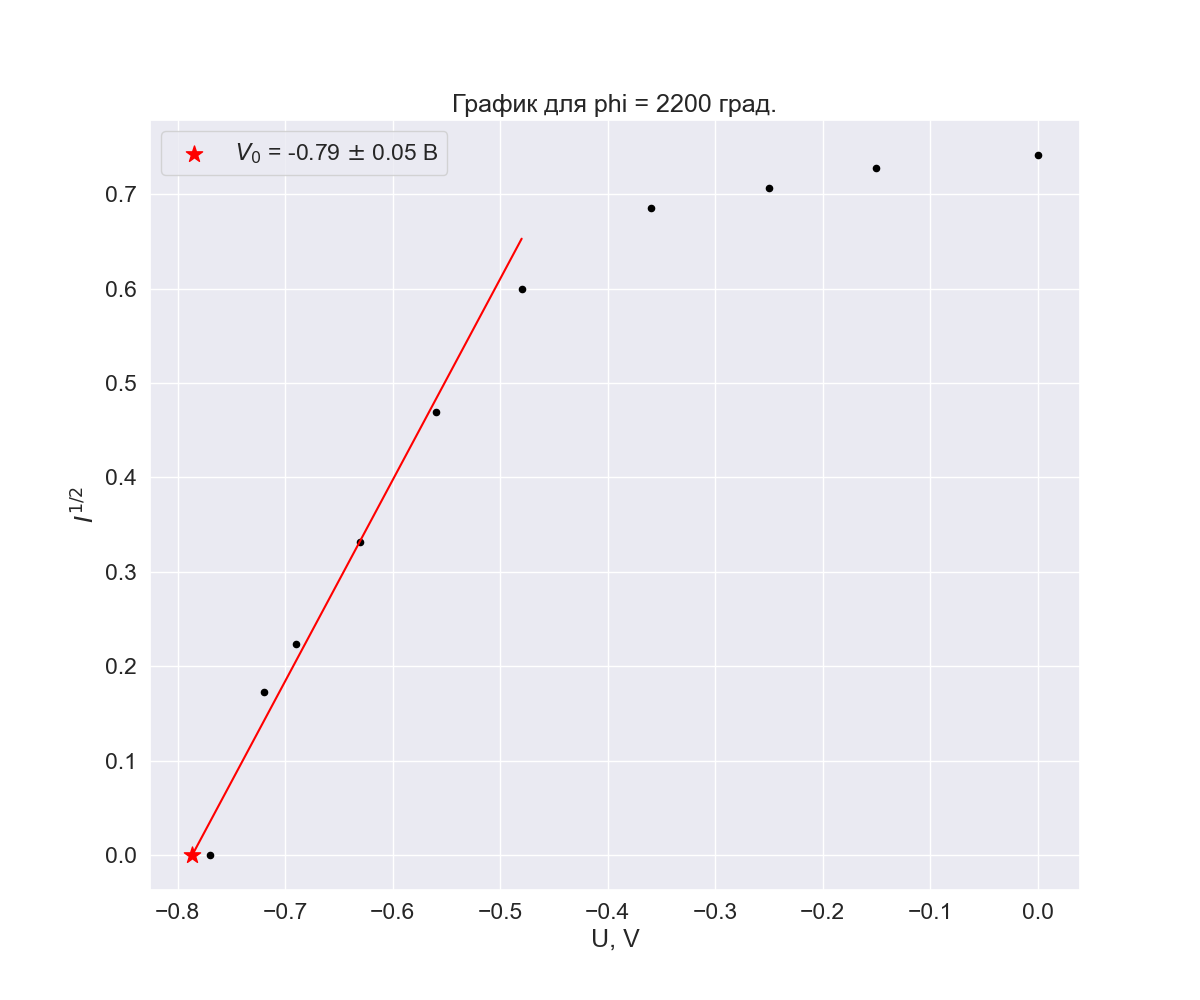
\includegraphics[width=1\textwidth]{plot_zero1.png}
    \caption{График для запирающего напряжения}
\end{figure}

\begin{figure}[H]
    \centering
    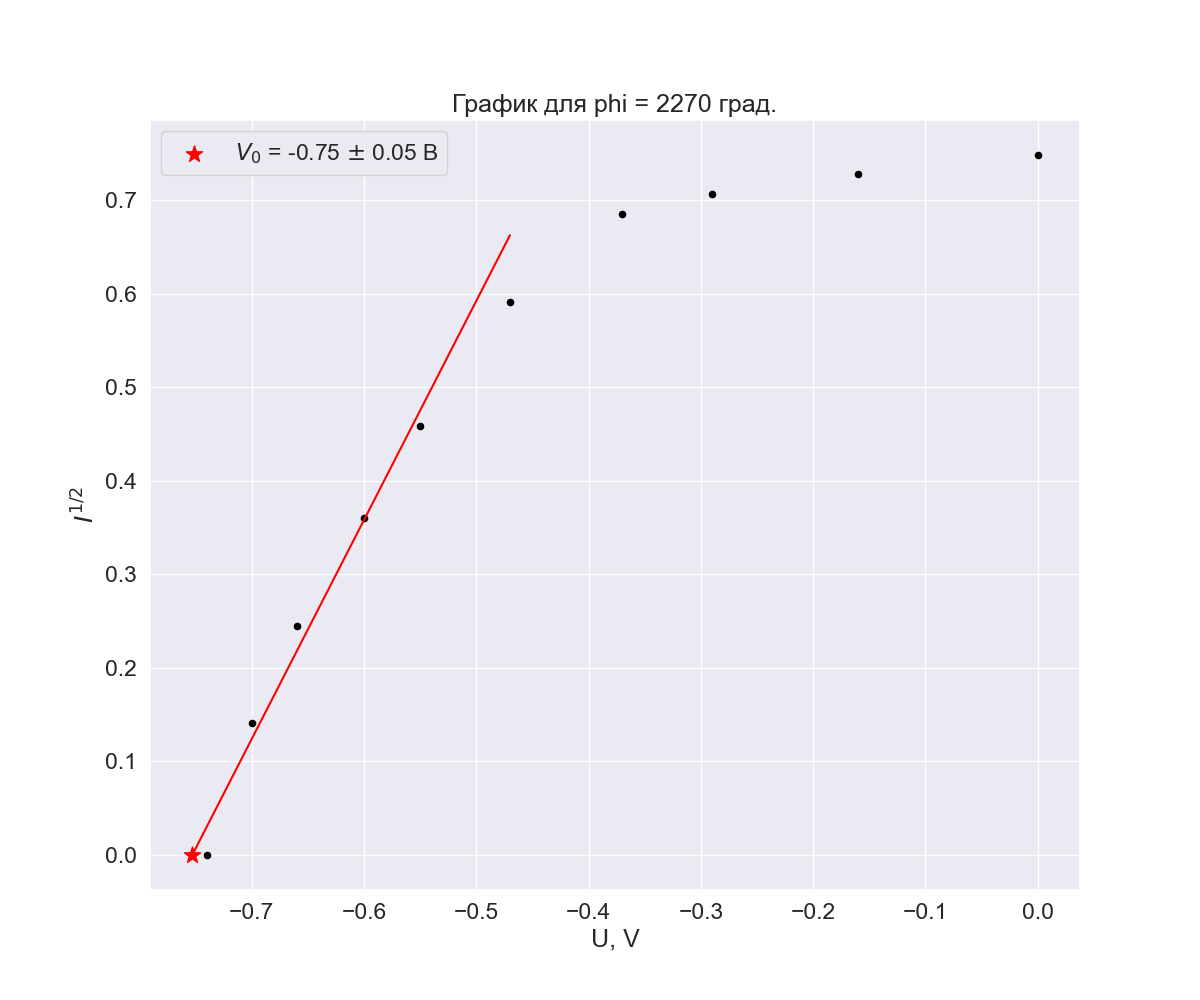
\includegraphics[width=1\textwidth]{plot_zero2.png}
    \caption{График для запирающего напряжения}
\end{figure}

\begin{figure}[H]
    \centering
    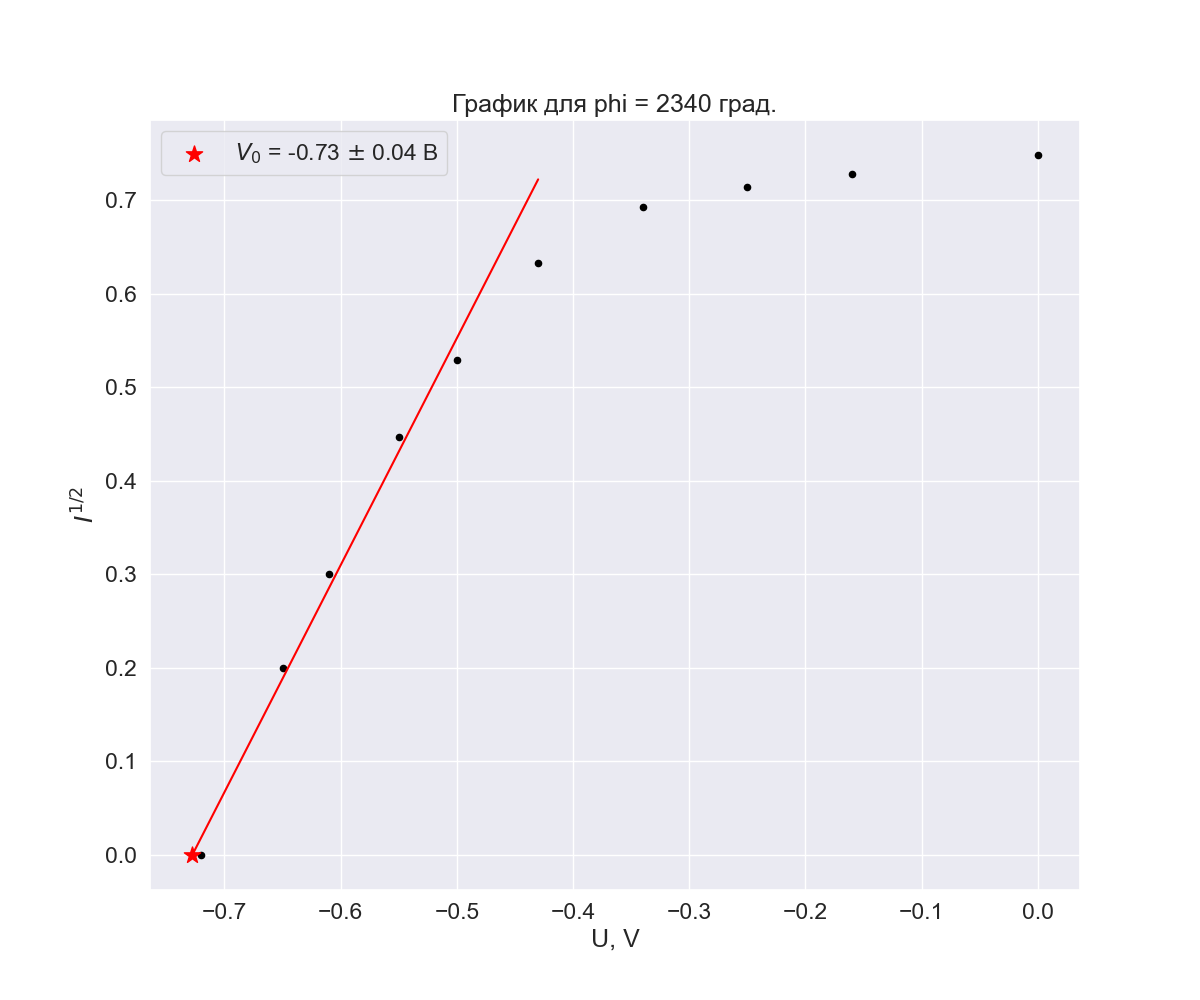
\includegraphics[width=1\textwidth]{plot_zero3.png}
    \caption{График для запирающего напряжения}
\end{figure}

\begin{figure}[H]
    \centering
    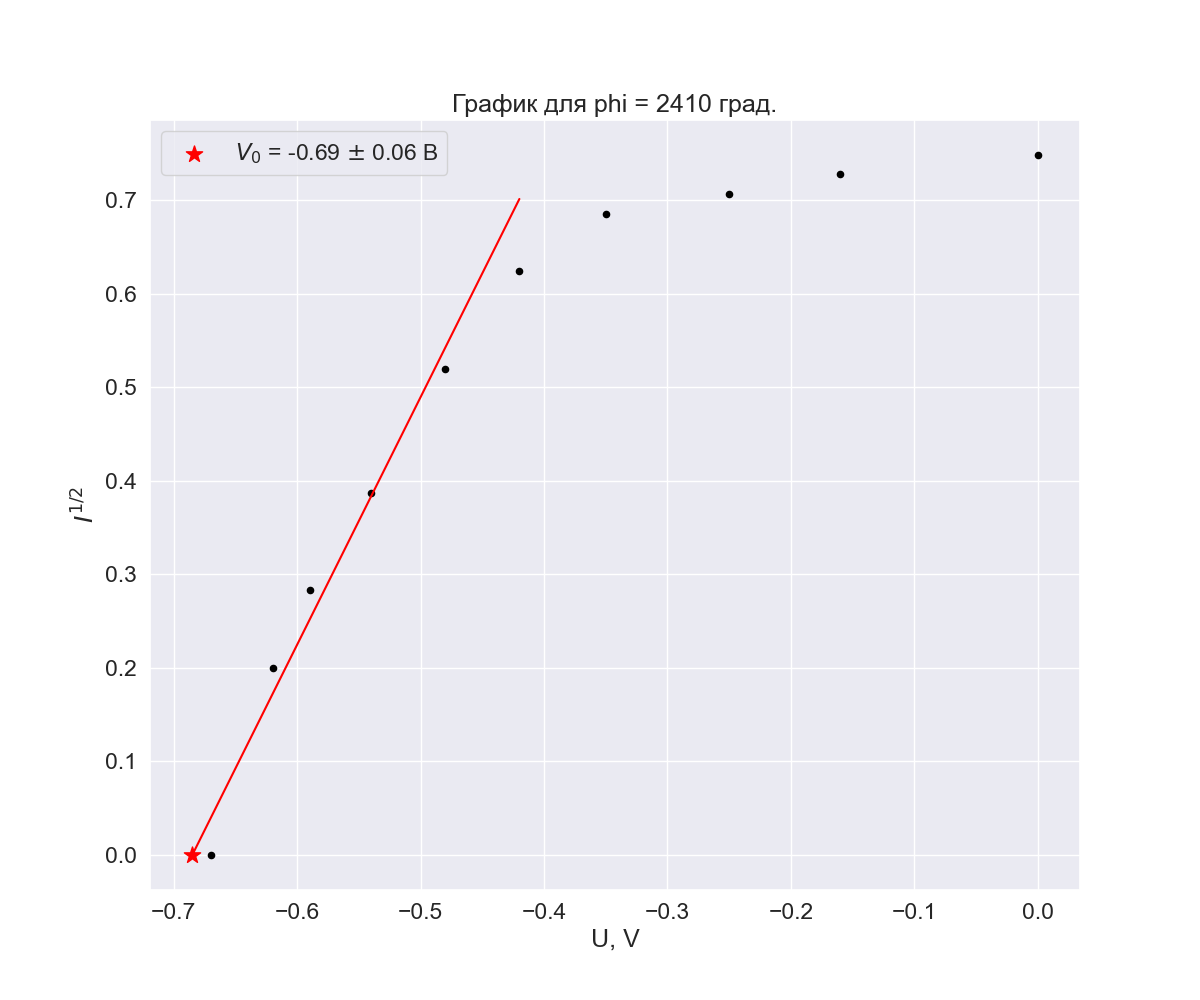
\includegraphics[width=1\textwidth]{plot_zero4.png}
    \caption{График для запирающего напряжения}
\end{figure}

\begin{figure}[H]
    \centering
    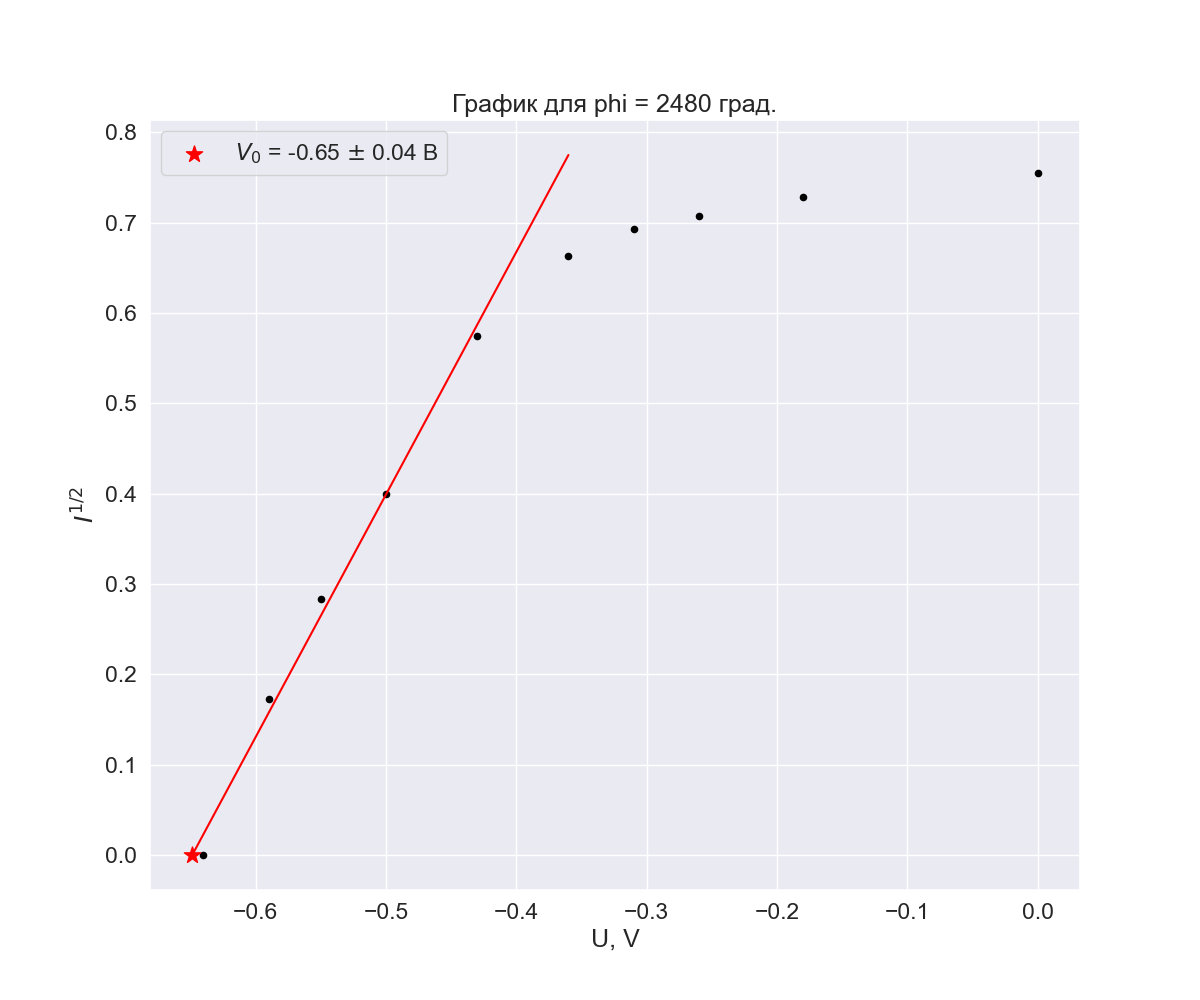
\includegraphics[width=1\textwidth]{plot_zero5.png}
    \caption{График для запирающего напряжения}
\end{figure}

\begin{figure}[H]
    \centering
    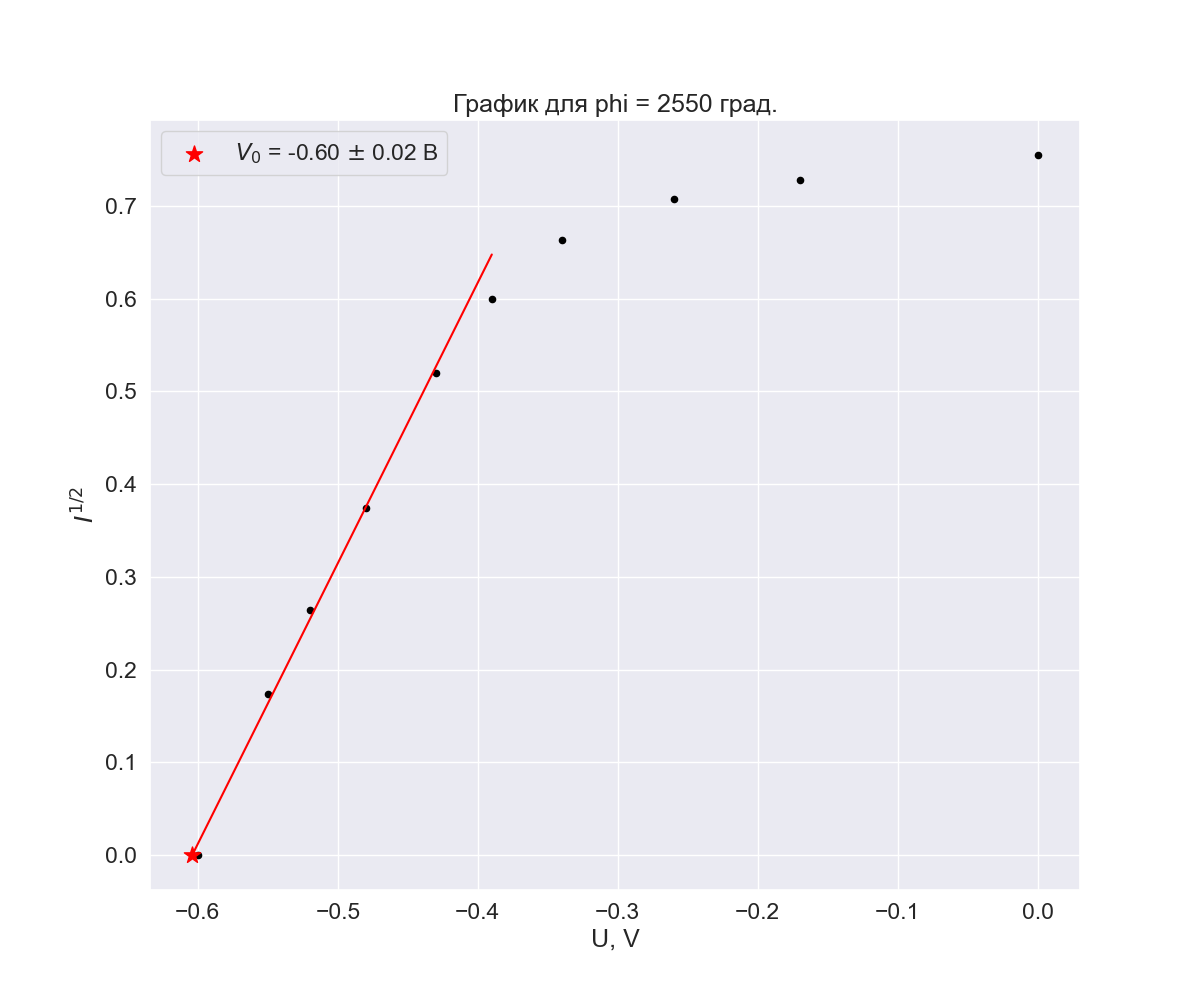
\includegraphics[width=1\textwidth]{plot_zero6.png}
    \caption{График для запирающего напряжения}
\end{figure}

\begin{figure}[H]
    \centering
    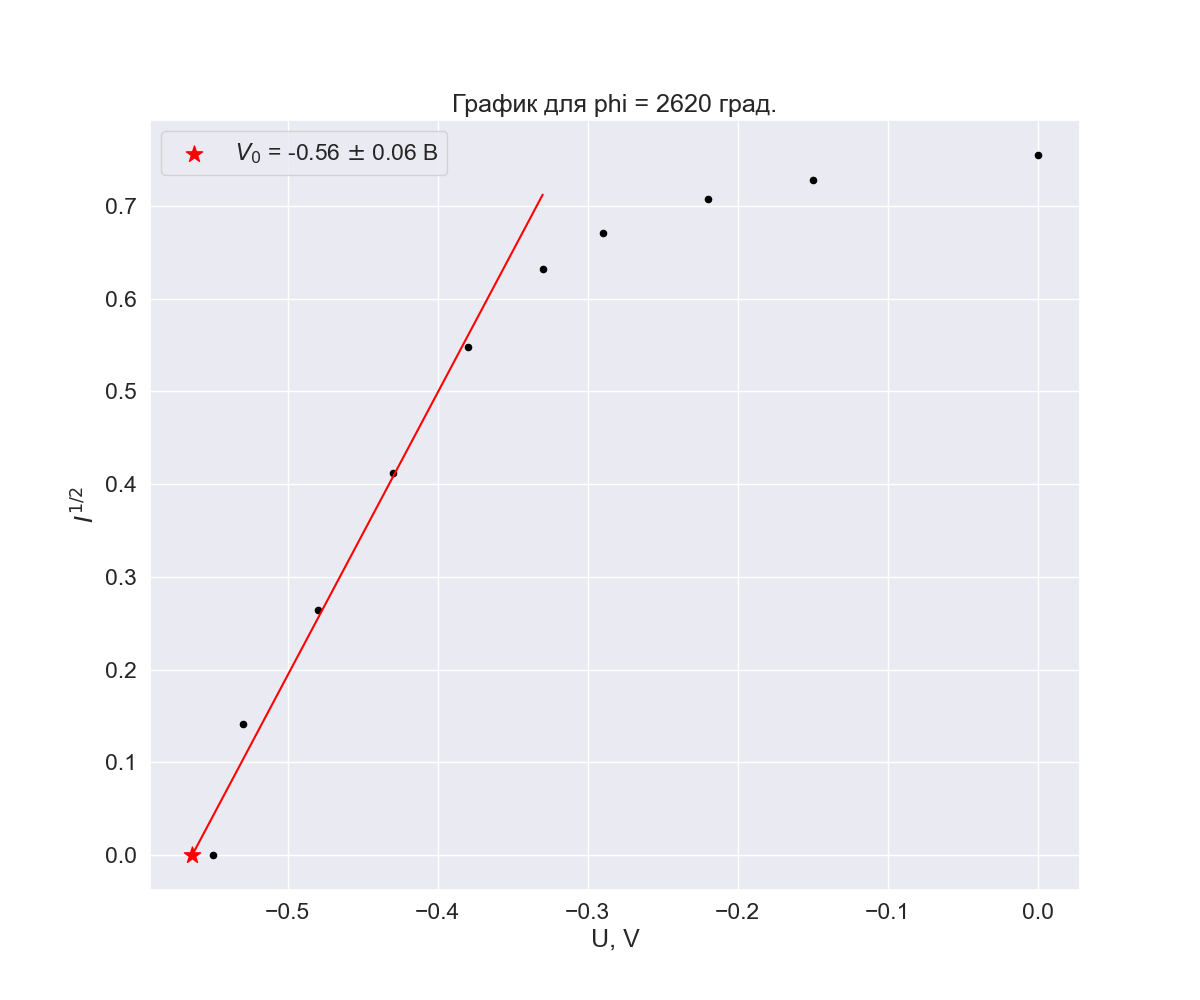
\includegraphics[width=1\textwidth]{plot_zero7.png}
    \caption{График для запирающего напряжения}
\end{figure}

\begin{figure}[H]
    \centering
    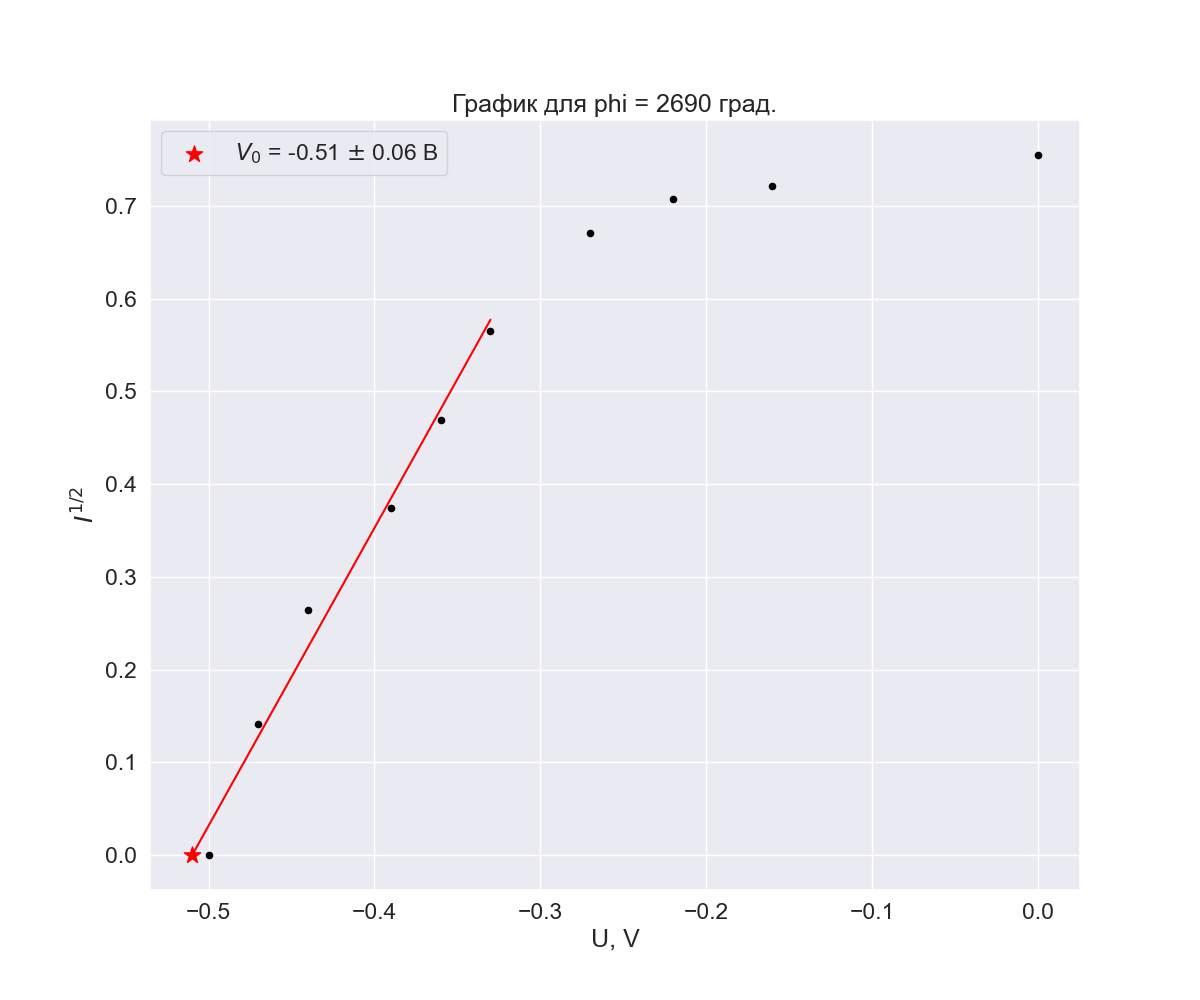
\includegraphics[width=1\textwidth]{plot_zero8.png}
    \caption{График для запирающего напряжения}
\end{figure}

\begin{figure}[H]
    \centering
    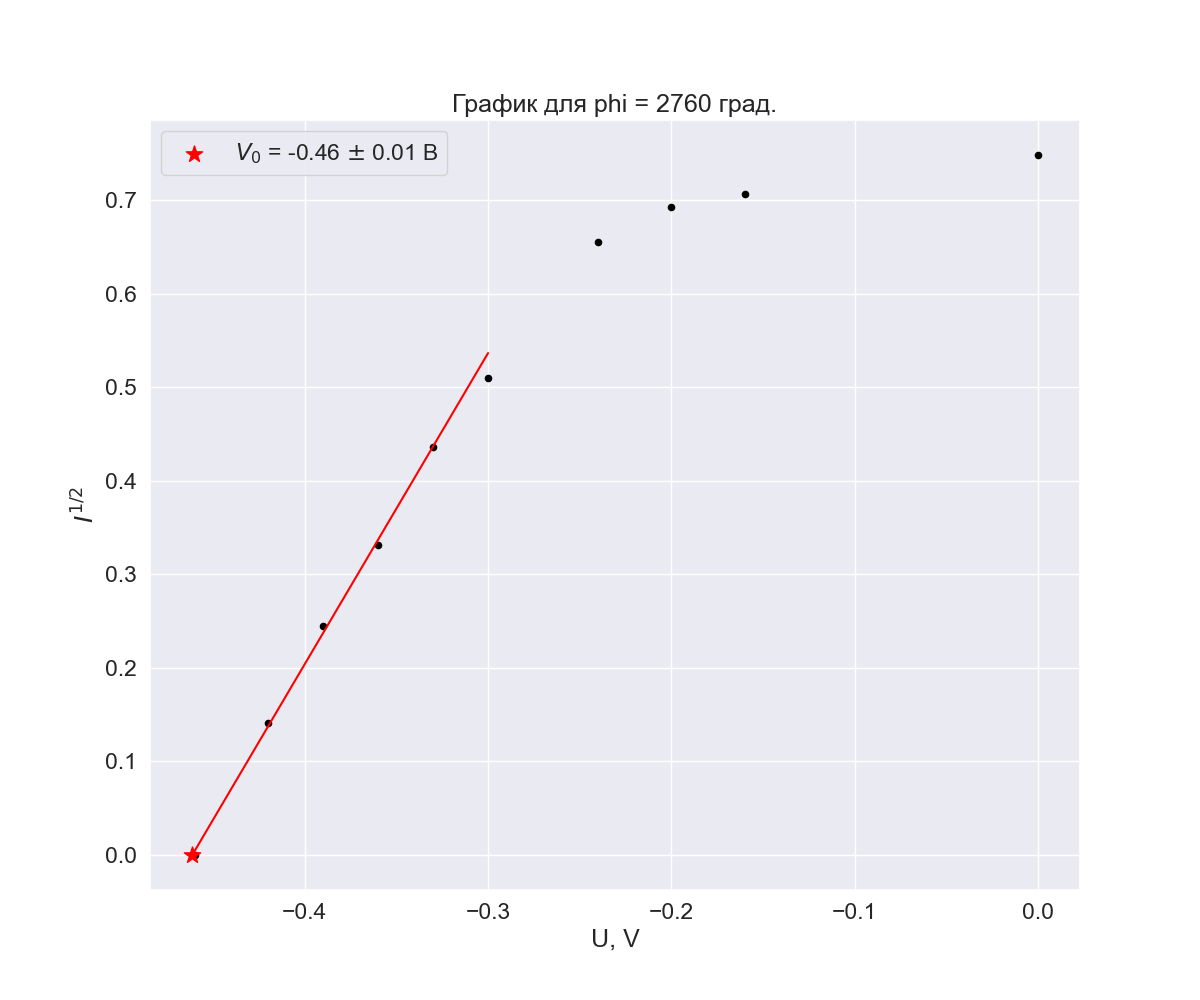
\includegraphics[width=1\textwidth]{plot_zero9.png}
    \caption{График для запирающего напряжения}
\end{figure}

\begin{figure}[H]
    \centering
    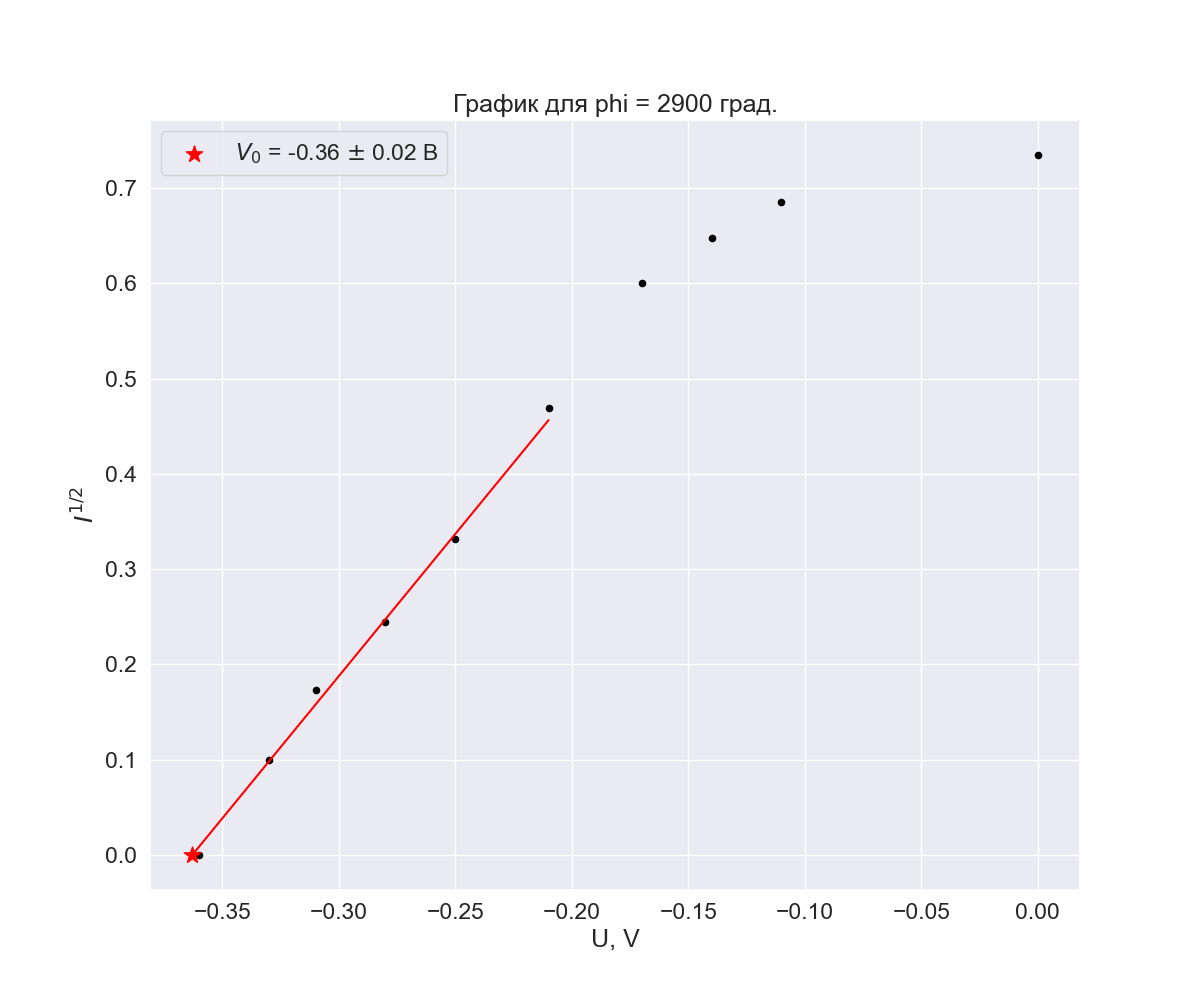
\includegraphics[width=1\textwidth]{plot_zero10.png}
    \caption{График для запирающего напряжения}
\end{figure}

\section{Выводы}


\end{document}